%!TEX encoding = UTF-8 Unicode
% !TeX spellcheck = en_GB
%%%%%%%%%%%%%%%%%%%%%%%%%%%%%%%%%%%%%%
\chapter{ Two-parameter fits of four-fermion operators and $C_\phi$ for HL-LHC}\label{app:hz}
%%%%%%%%%%%%%%%%%%%%%%%%%%%%%%%%%%%%%%
\label{app:due}
I present here in~\autoref{2param-cqthl} and ~\autoref{2param-cqtqbhl} the fit results for the SMEFT four heavy quark operators with the Higgs trilinear self-coupling modifier $C_\phi$ for the HL-LHC projections by CMS~\cite{CMS-PAS-FTR-18-011,twiki} as an extension of the results presented in~\autoref{chap:4topSingleHiggs}.\\
\begin{figure}[htpb!]
	\vspace{-0.7 cm}
\begin{center}
	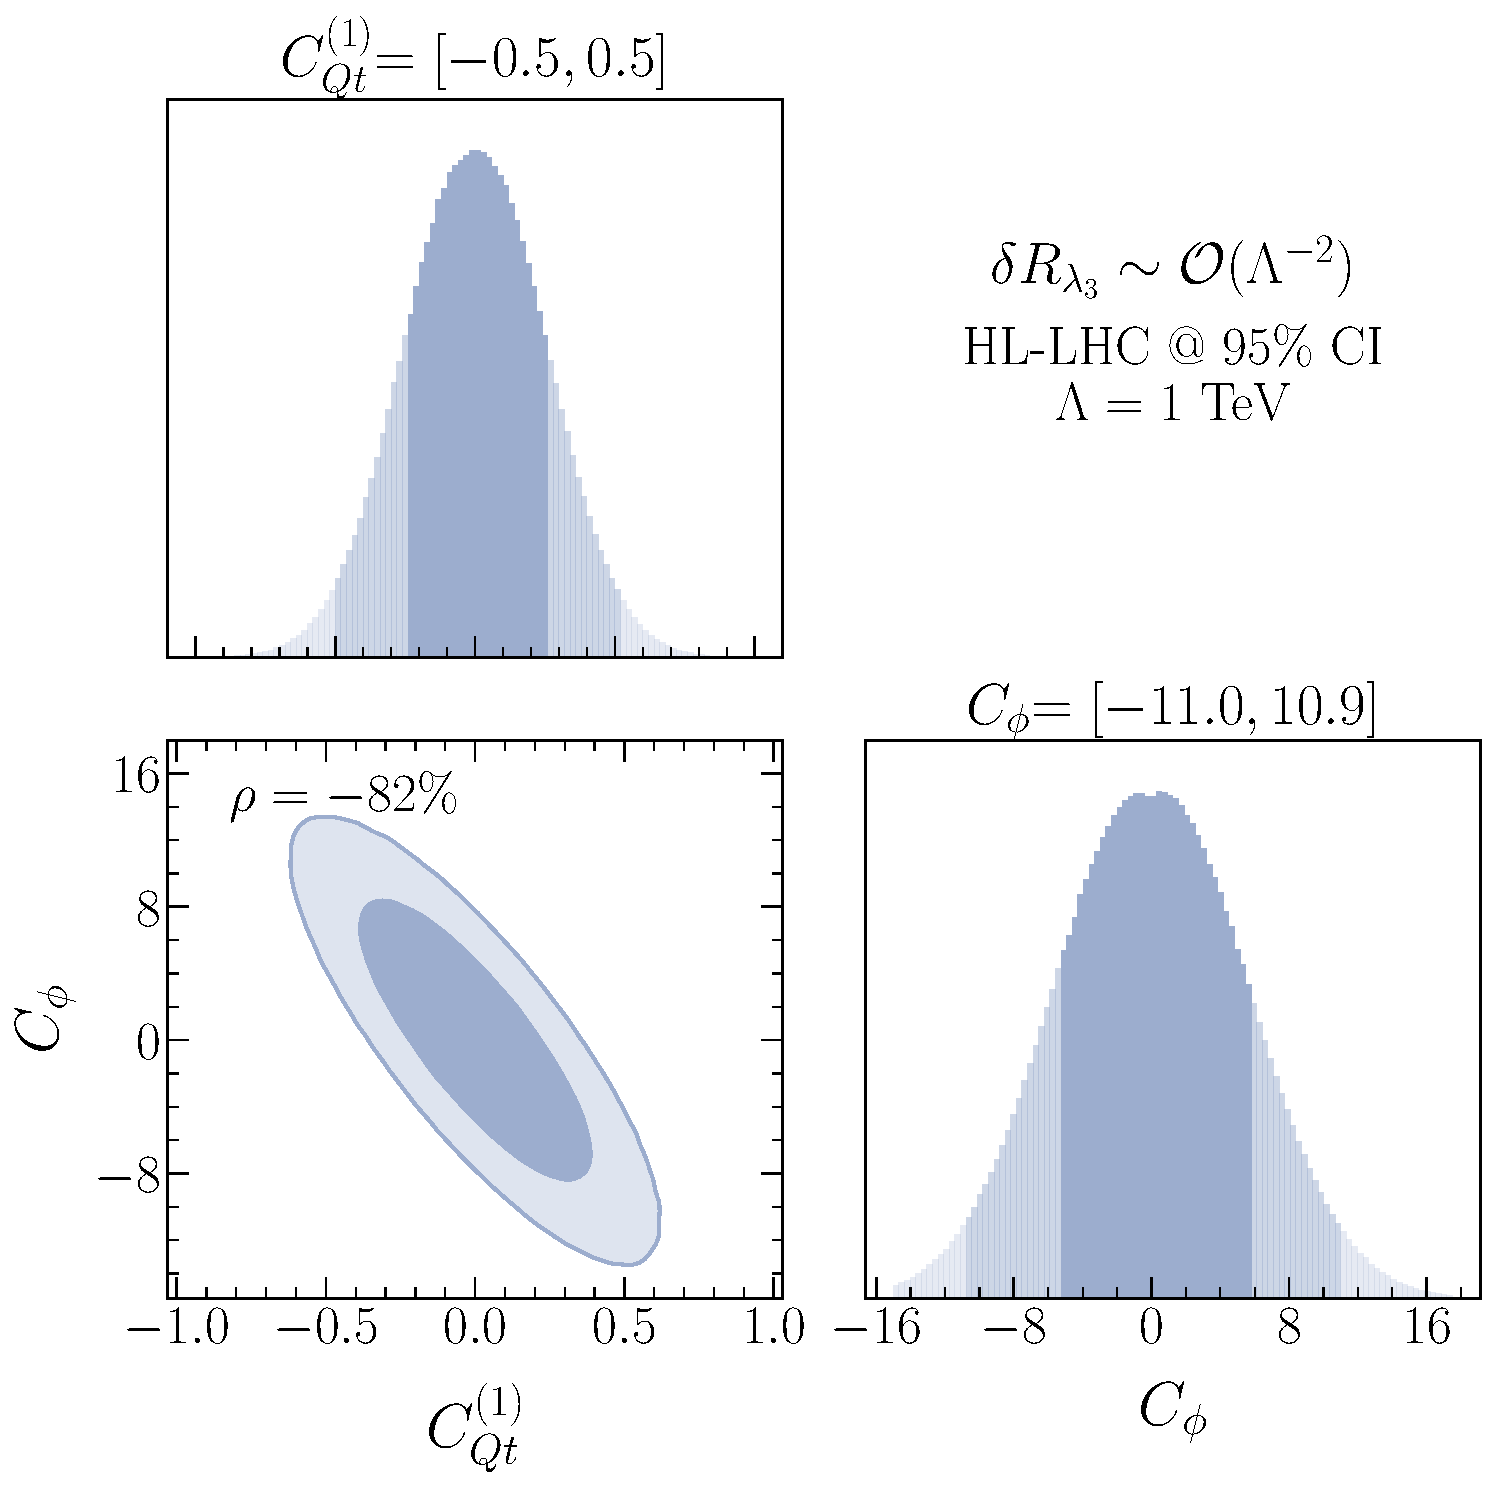
\includegraphics[width=0.4\linewidth]{figures/hl-lhc/Cqt1_HL-LHC_linearl3_rge}
	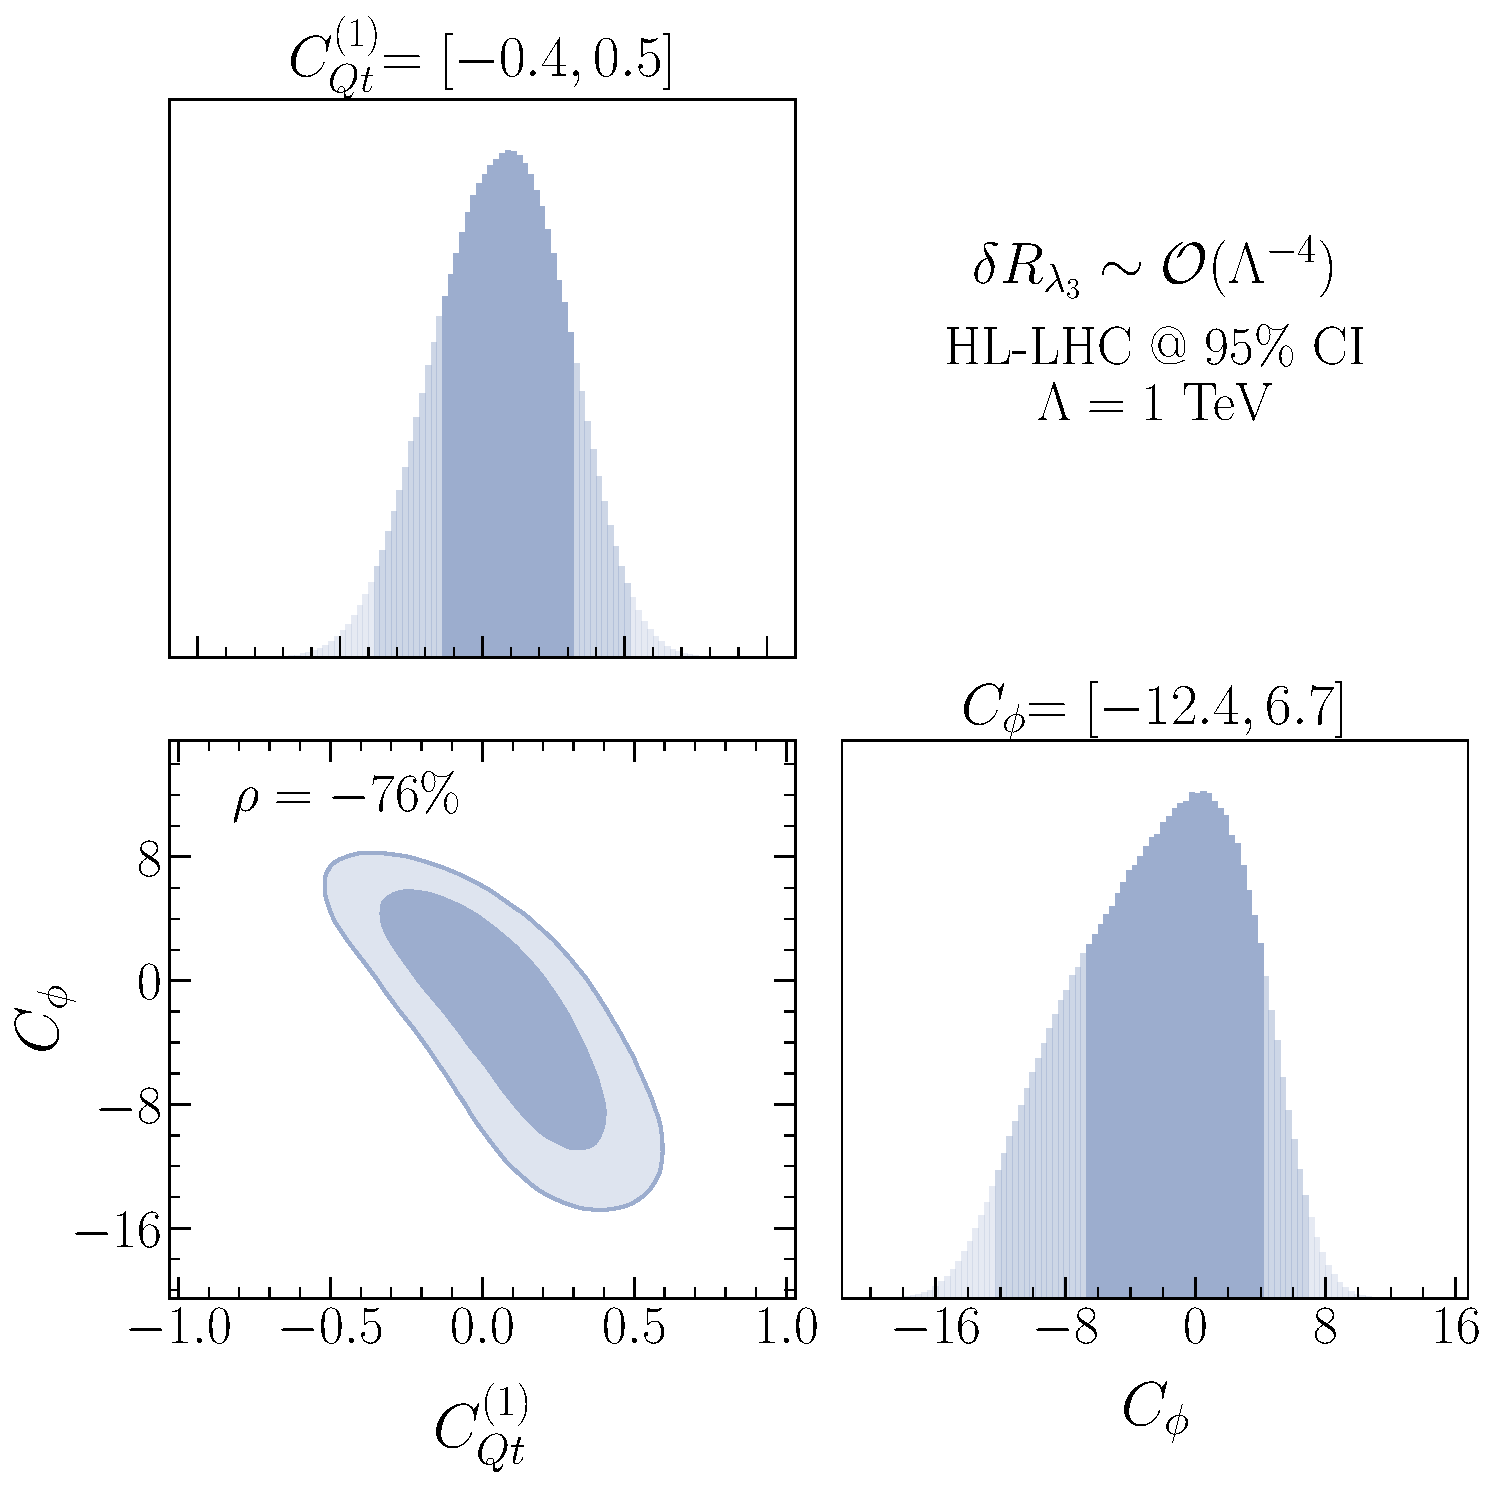
\includegraphics[width=0.4\linewidth]{figures/hl-lhc/Cqt1_HL-LHC_quadl3_rge} \\ 
	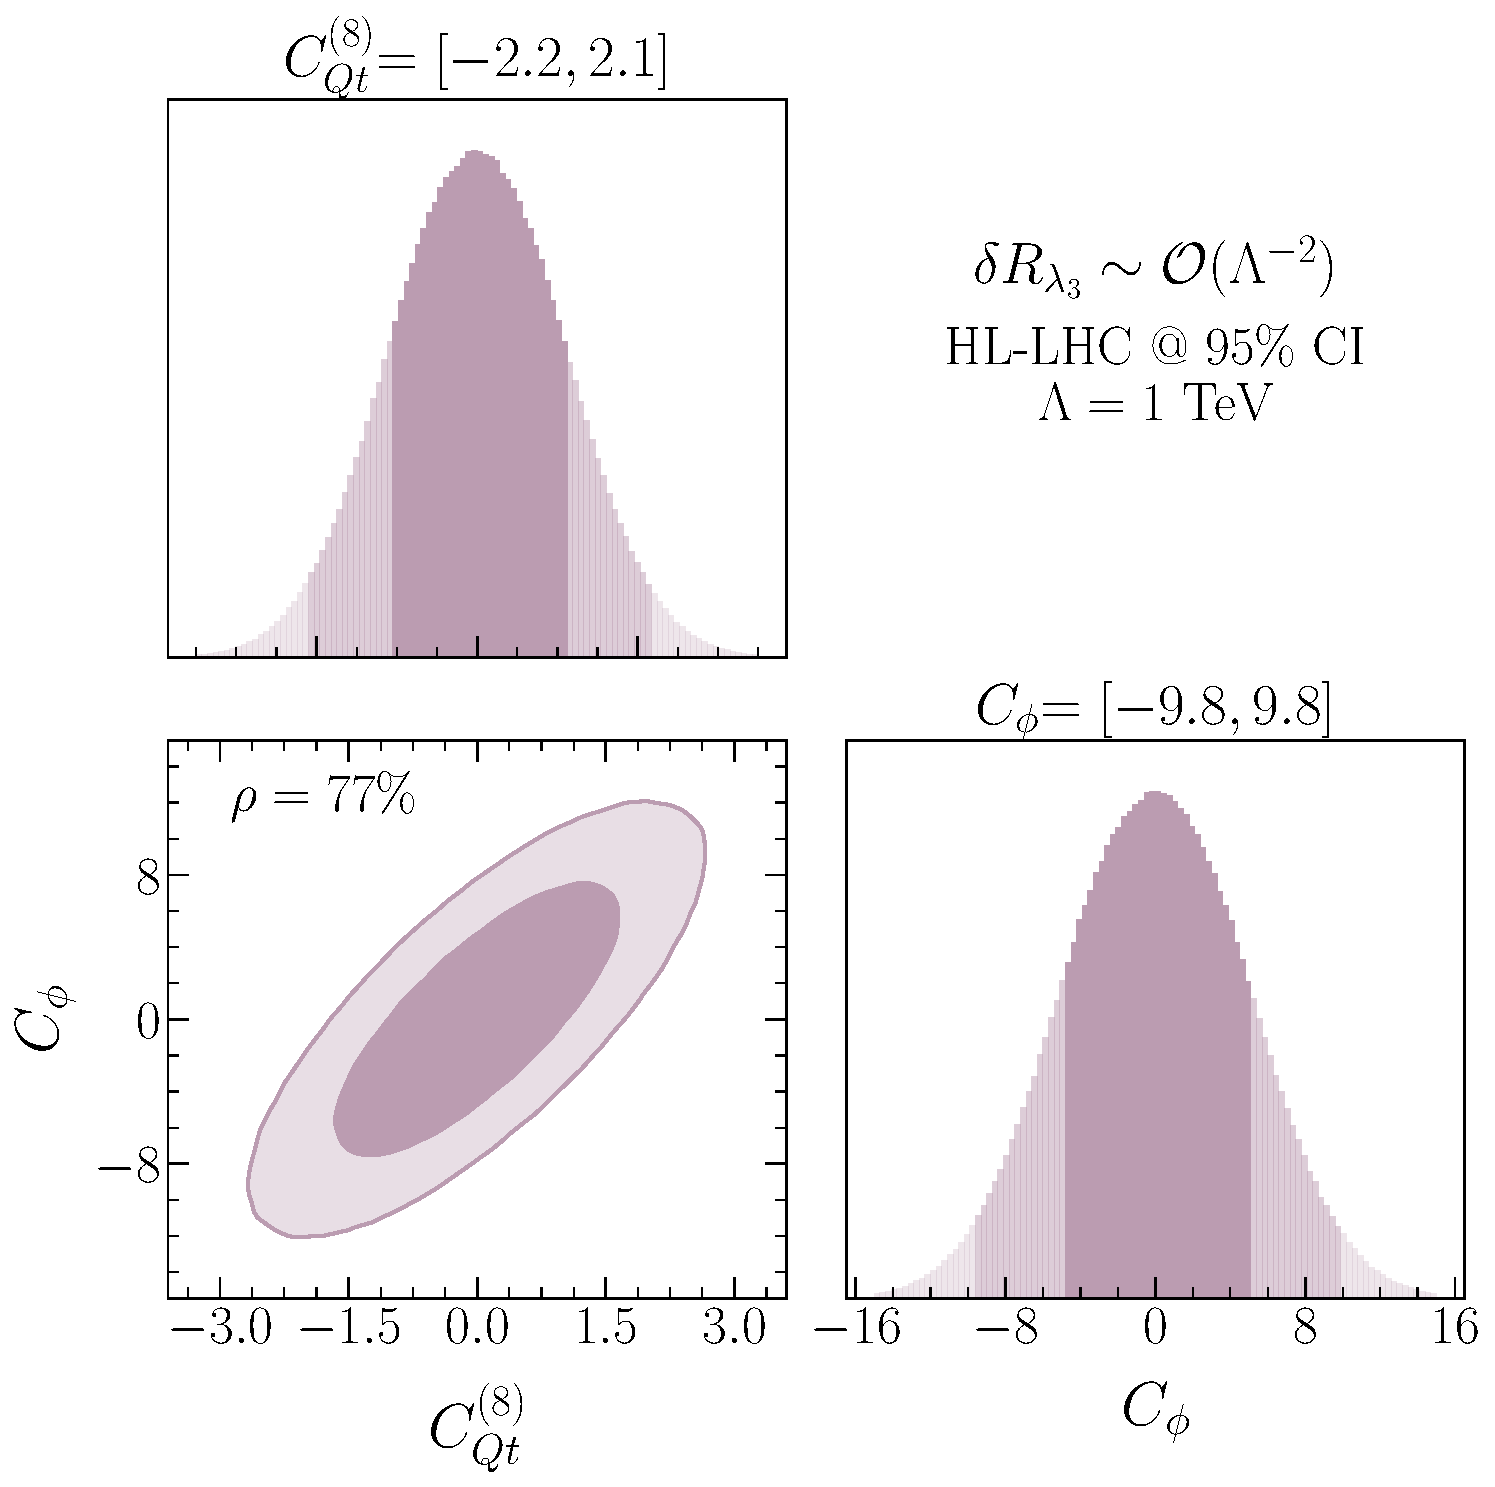
\includegraphics[width=0.4\linewidth]{figures/hl-lhc/Cqt8_LHL-LHC_linearl3_rge}
	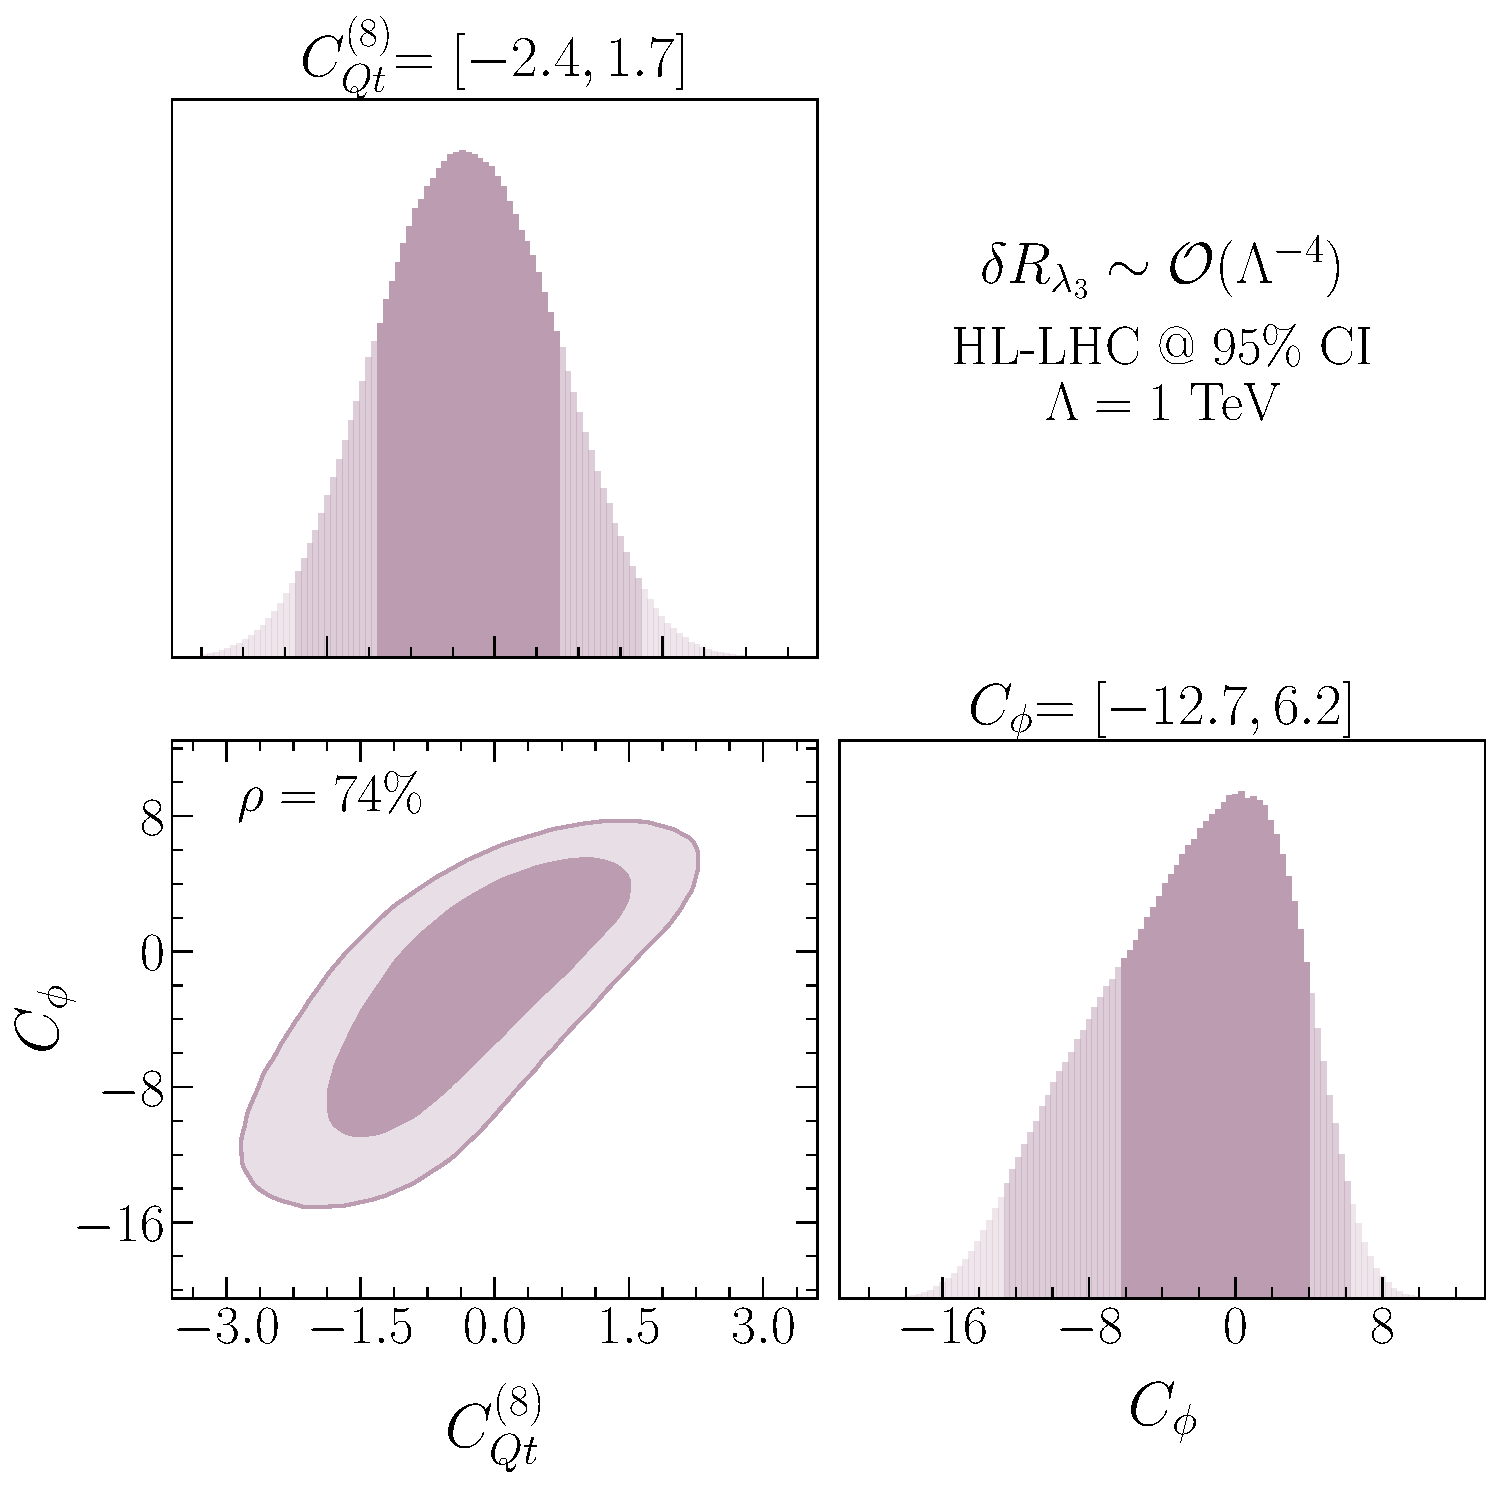
\includegraphics[width=0.4\linewidth]{figures/hl-lhc/Cqt8_HL-LHC_quadl3_rge} 
\end{center}
\caption{The posterior distributions of the HL-LHC projections fits for $C_\phi$ with $C_{Qt}^{(1)}$ (up) and $C_\phi$ with $C_{Qt}^{(8)}$ (down). With 68\% and 95\% highest density posterior contours indicated. The limits shown on top of the plots indicate the 95\% CI's. Plots on the left are made for the fully linearised n $\delta R_{\lambda_3}$, while the ones on the right include the quadratic effects.  \label{2param-cqthl}   }
\end{figure}
The expected constraints improve from the Run-II ones by a factor of 
\be
 \sim\sqrt{\mathscr{L}_{\rm HL-LHC}\over \mathscr{L}_{\rm Run-II} },
\ee
as expected, from statistical analysis. This comes from the adaptation of the $S_2$ uncertainties scheme.  \\ The linear fits show similar correlation patters to the ones from the Run-II in~\autoref{2param-cqt} and ~\autoref{2param-cqtqb}. However, the quadratic $R_{\lambda_3}$ scheme shows strong correlation between $C_\phi$ and the four-heavy quark Wilson coefficients, while this is not seen in the Run-II fits. The implication of these correlations is worsened projected constraints on negative $C_\phi$ values in the two-parameter fits. 
\begin{figure}[htpb!]
\begin{center}
	\begin{center}
		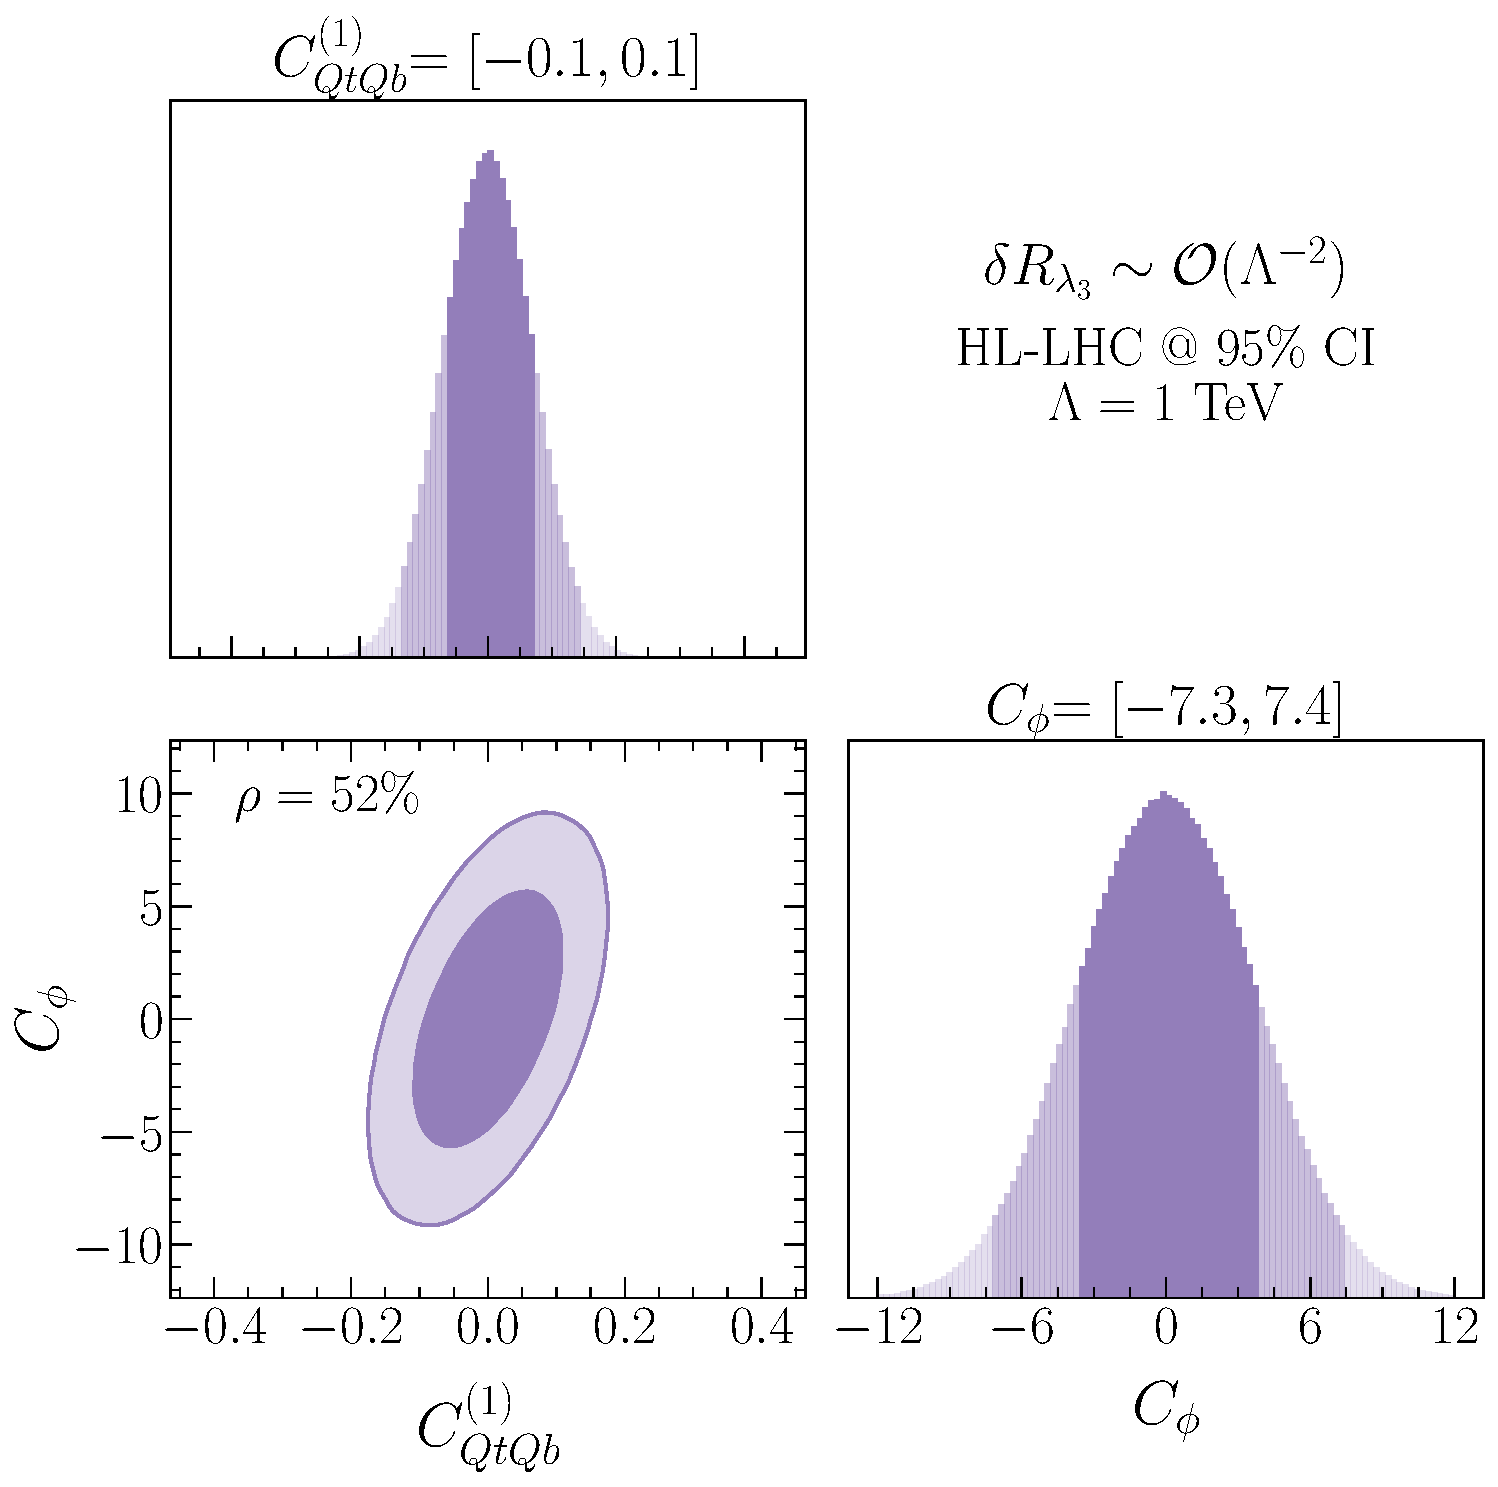
\includegraphics[width=0.4\linewidth]{figures/hl-lhc/Cqtqb1_HL-LHC_linearl3_rge}
		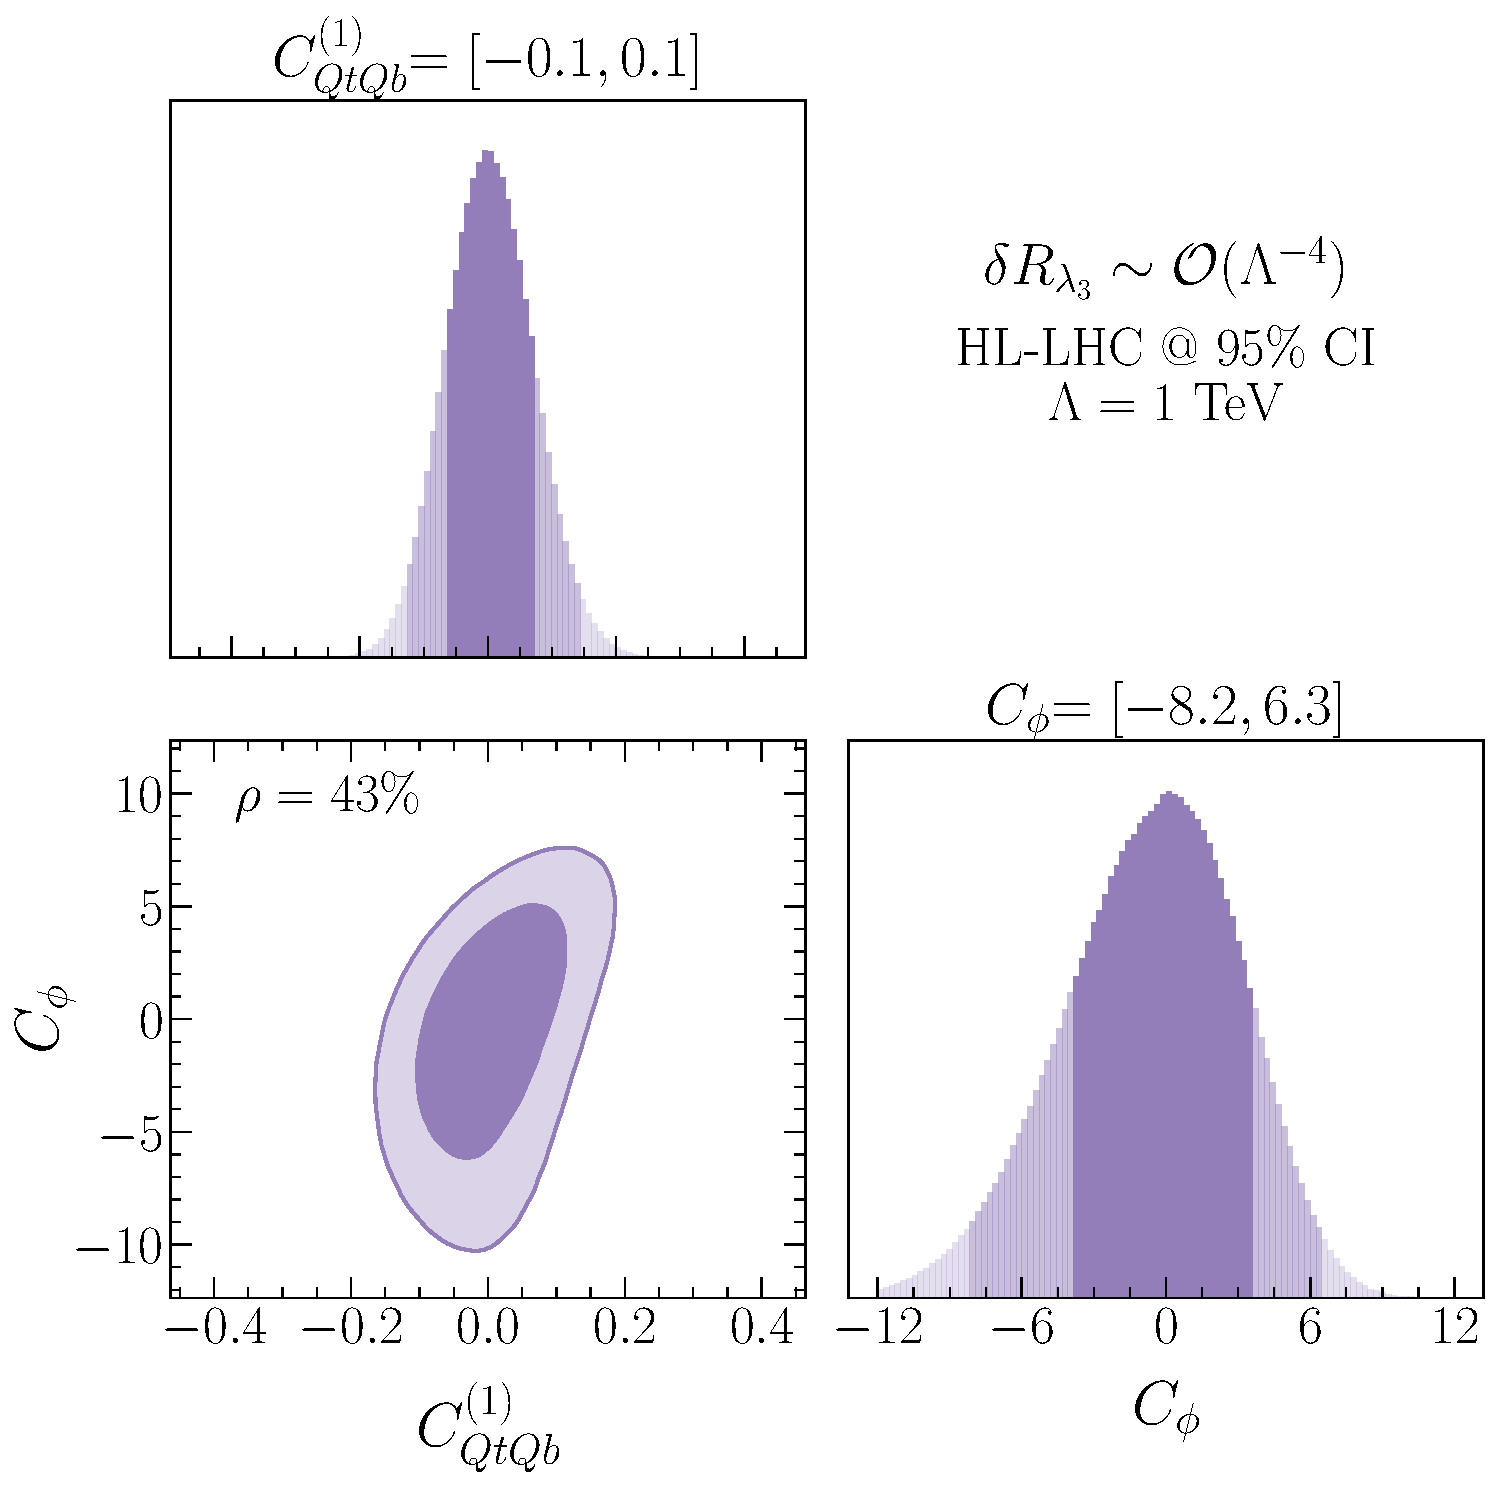
\includegraphics[width=0.4\linewidth]{figures/hl-lhc/Cqtqb1_HL-LHC_quadl3_rge} \\ 
		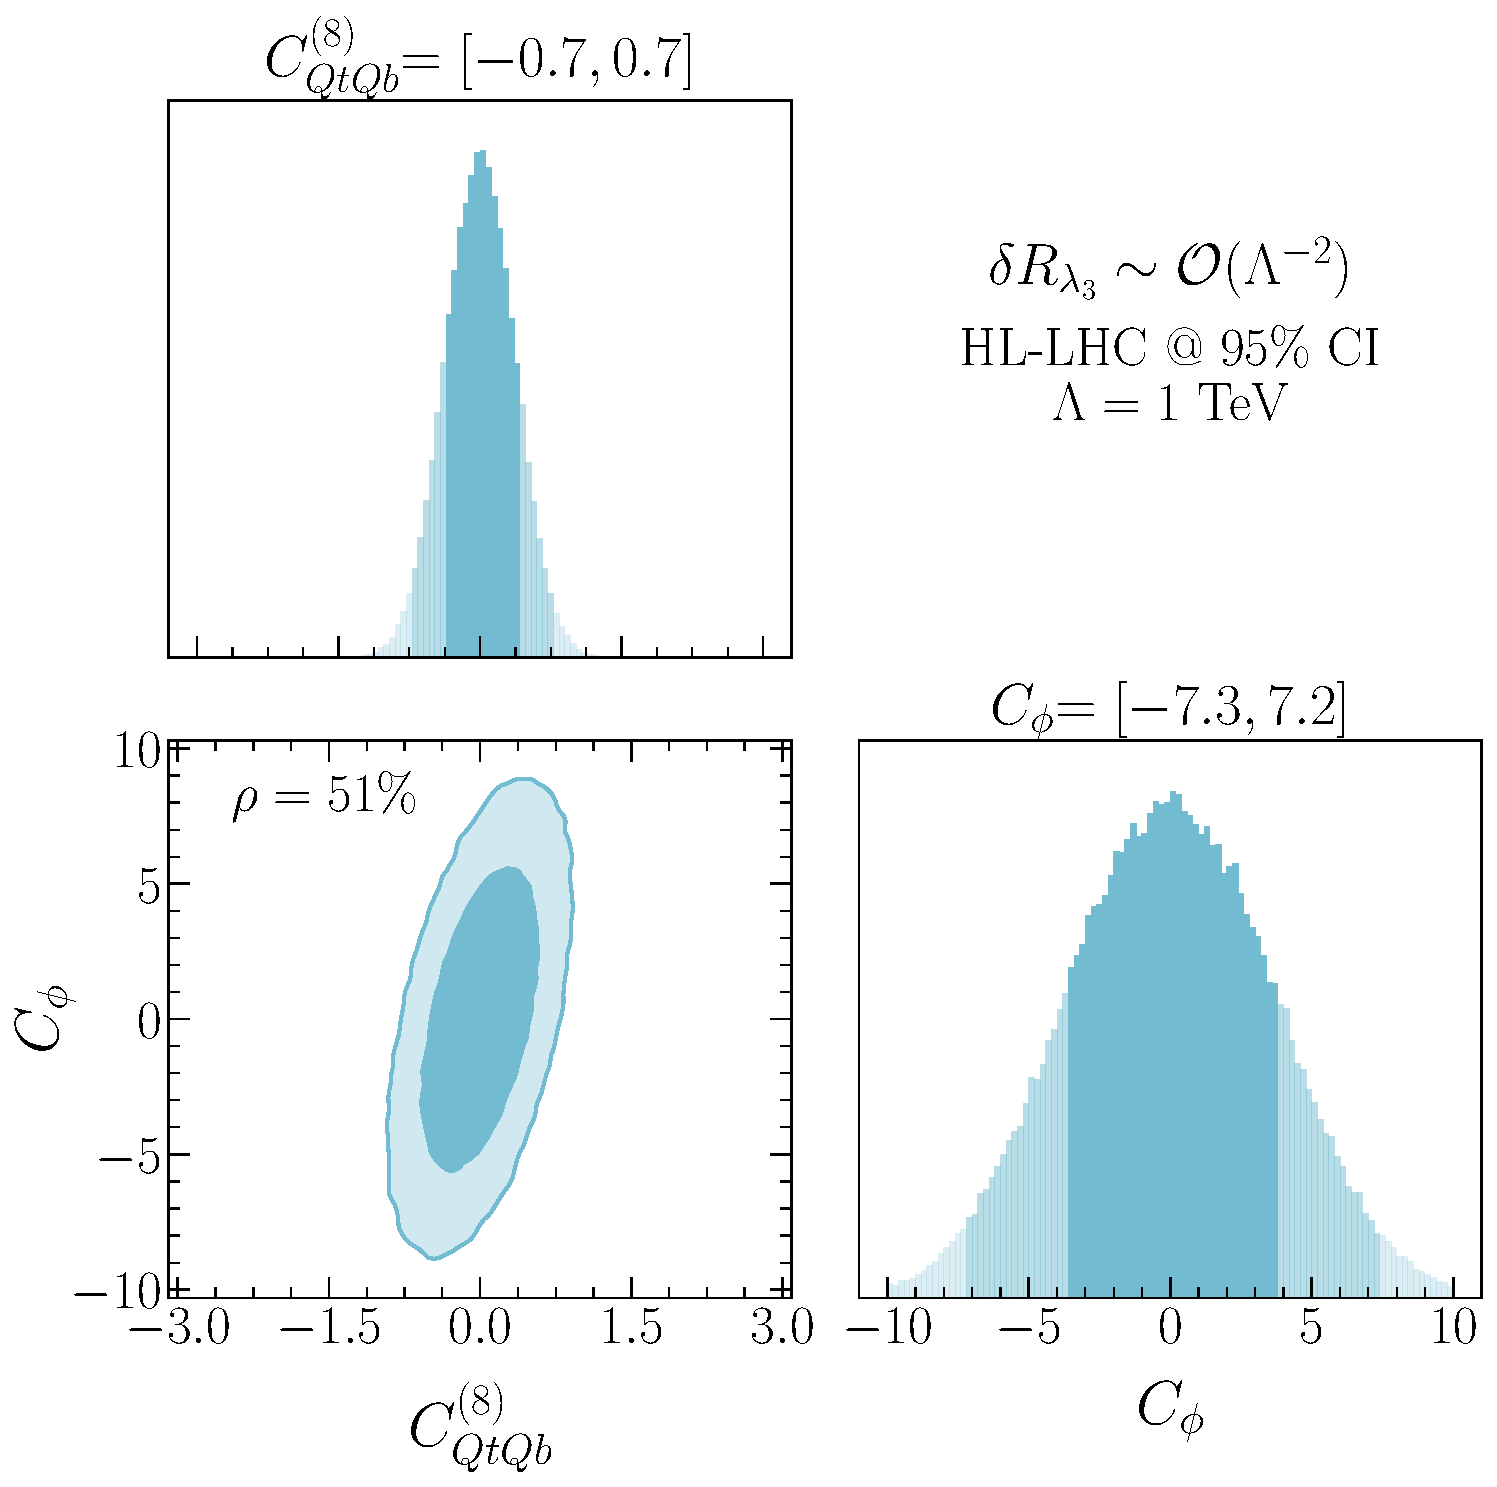
\includegraphics[width=0.4\linewidth]{figures/hl-lhc/Cqtqb8_HL-LHC_linearl3_rge}
		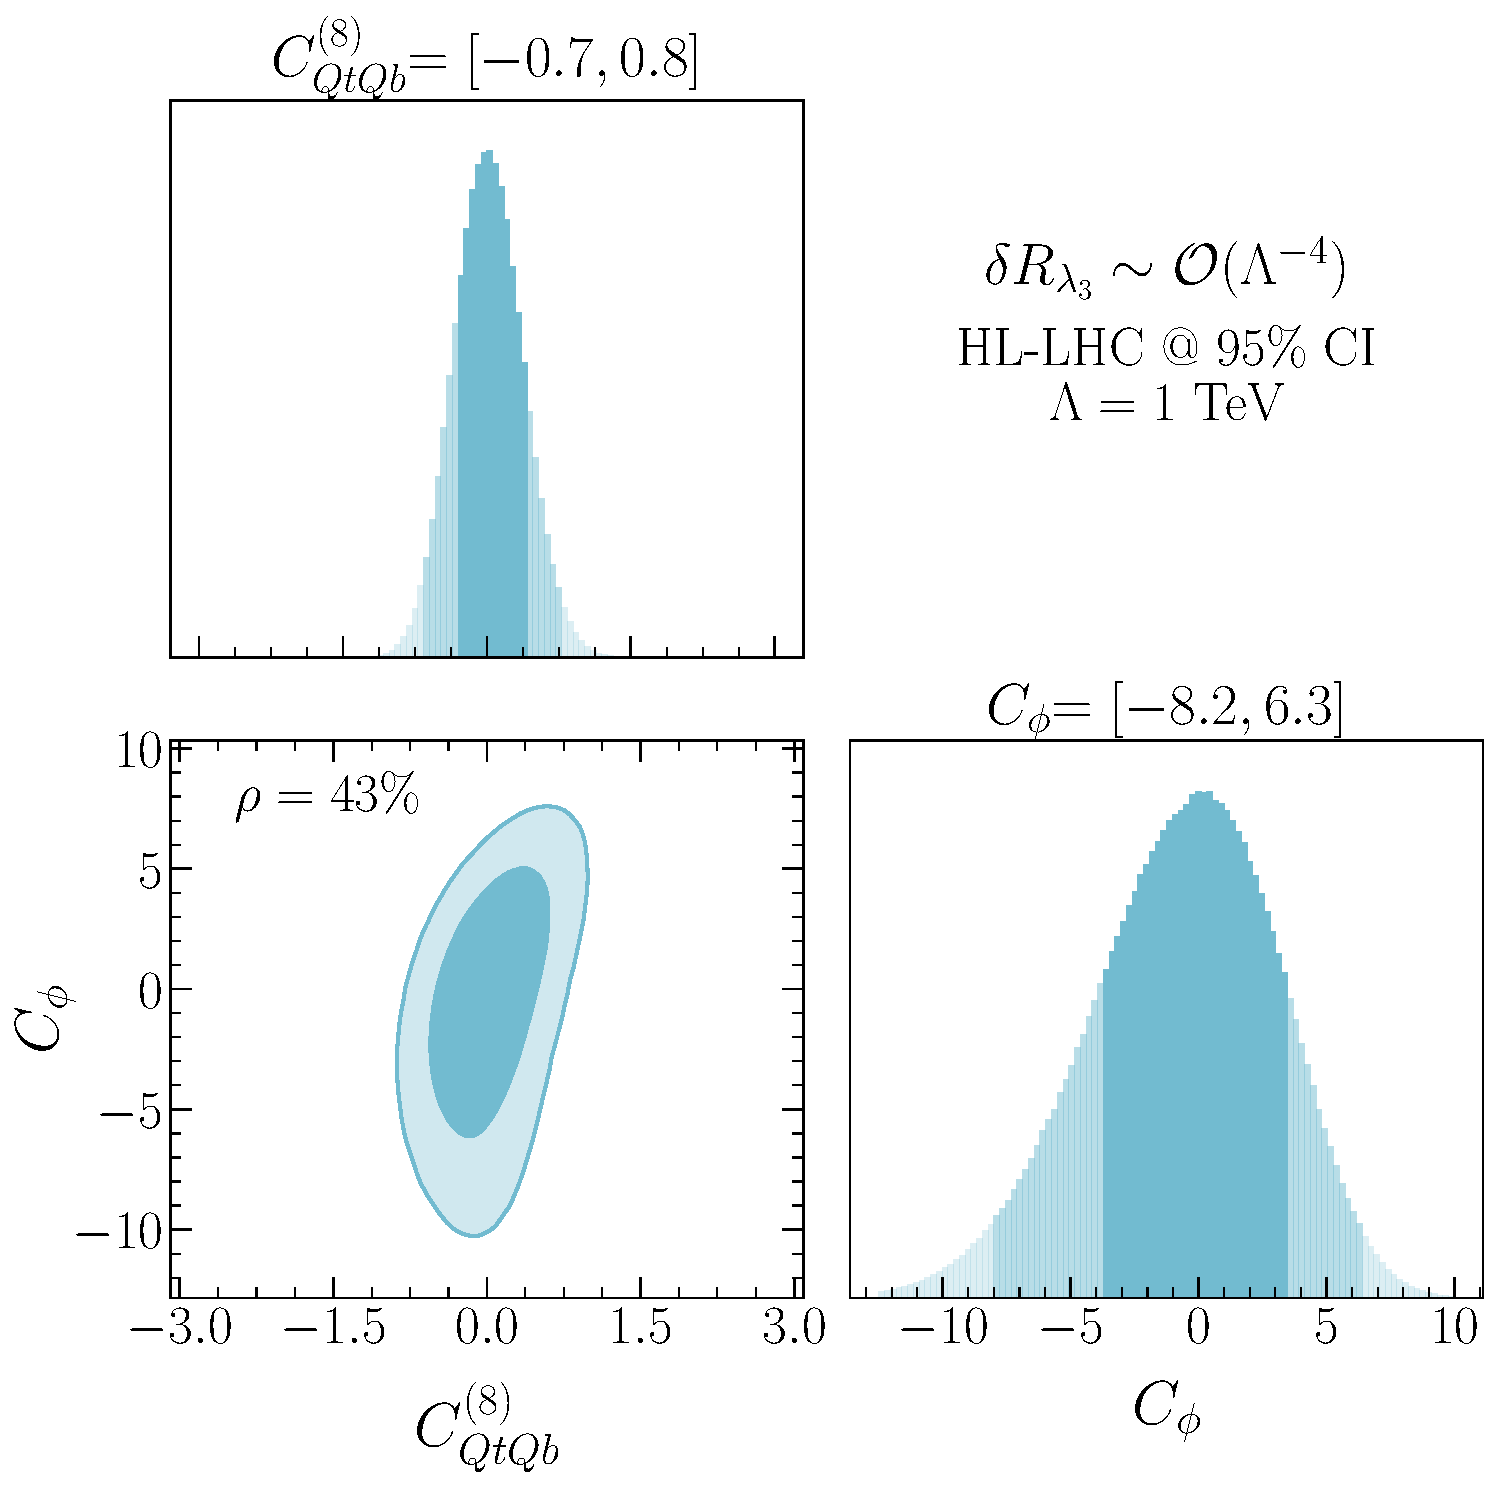
\includegraphics[width=0.4\linewidth]{figures/hl-lhc/Cqtqb8_HL-LHC_quadl3_rge} 
	\end{center}
\end{center}
\caption{The posterior distributions of the HL-LHC projections fits for $C_\phi$ with $C_{QtQb}^{(1)}$ (up) and $C_\phi$ with $C_{QtQb}^{(8)}$ (down). With the same annotations as in~\autoref{2param-cqthl}.  \label{2param-cqtqbhl}}
\end{figure}